% Graph paper
% Author: Benjamin Abel
% https://texample.net/tikz/examples/graph-paper/
\documentclass{article}
\usepackage{geometry}
\geometry{hmargin=1cm,vmargin=1cm}
\usepackage{tikz}
\def\width{18}
\def\hauteur{13}

\begin{document}

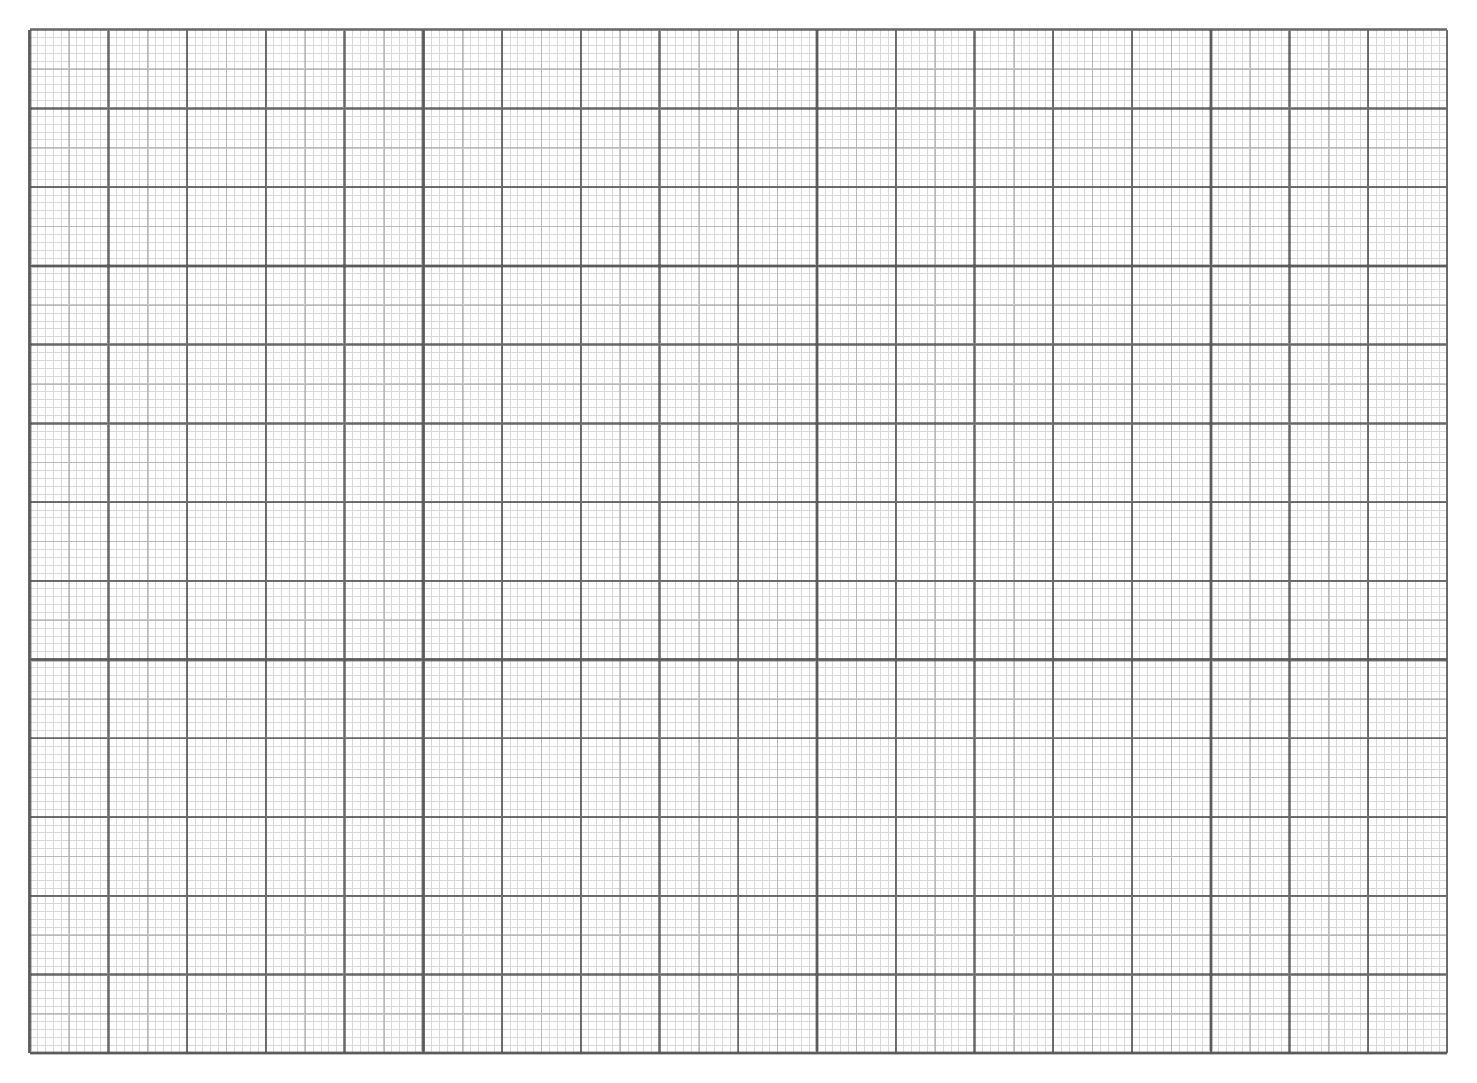
\begin{tikzpicture}[x=1cm, y=1cm, semitransparent]
\draw[step=1mm, line width=0.1mm, black!30!white] (0,0) grid (\width,\hauteur);
\draw[step=5mm, line width=0.2mm, black!40!white] (0,0) grid (\width,\hauteur);
\draw[step=5cm, line width=0.5mm, black!50!white] (0,0) grid (\width,\hauteur);
\draw[step=1cm, line width=0.3mm, black!90!white] (0,0) grid (\width,\hauteur);
\end{tikzpicture}

\end{document}
